\documentclass[tikz,dvipsnames]{standalone}

\usepackage{amsmath}


\begin{document}
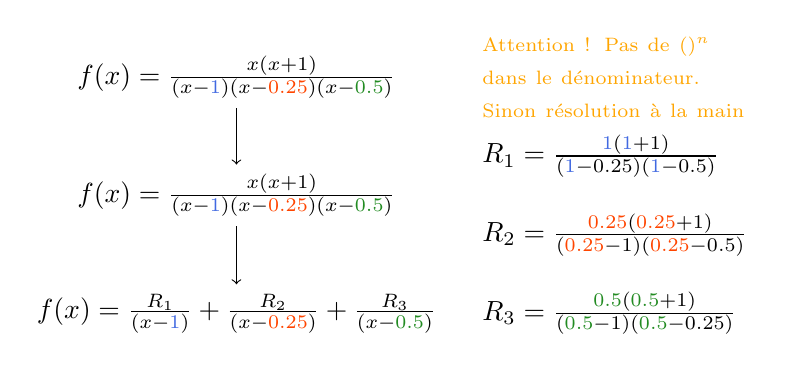
\begin{tikzpicture}
\node (A) at (0,1) {$f(x)=\frac{x(x+1)}{(x-\textcolor{RoyalBlue}{1})(x-\textcolor{OrangeRed}{0.25})(x-\textcolor{ForestGreen}{0.5})}$};
\node[text width=3.5cm,anchor=west,Orange] at (3,1) {\scriptsize Attention ! Pas de $()^n$ dans le dénominateur. Sinon résolution à la main};
\node (B) at (0,-0.5) {$f(x)=\frac{x(x+1)}{(x-\textcolor{RoyalBlue}{1})(x-\textcolor{OrangeRed}{0.25})(x-\textcolor{ForestGreen}{0.5})}$};
\node (C) at (0,-2) {$f(x)=\frac{R_1}{(x-\textcolor{RoyalBlue}{1})}+\frac{R_2}{(x-\textcolor{OrangeRed}{0.25})}+\frac{R_3}{(x-\textcolor{ForestGreen}{0.5})}$};
\node[anchor=west] (D) at (3,0) {$R_1=\frac{\textcolor{RoyalBlue}{1}(\textcolor{RoyalBlue}{1}+1)}{(\textcolor{RoyalBlue}{1}-0.25)(\textcolor{RoyalBlue}{1}-0.5)}$};
\node[anchor=west] (E) at (3,-1) {$R_2=\frac{\textcolor{OrangeRed}{0.25}(\textcolor{OrangeRed}{0.25}+1)}{(\textcolor{OrangeRed}{0.25}-1)(\textcolor{OrangeRed}{0.25}-0.5)}$};
\node[anchor=west] (F) at (3,-2) {$R_3=\frac{\textcolor{ForestGreen}{0.5}(\textcolor{ForestGreen}{0.5}+1)}{(\textcolor{ForestGreen}{0.5}-1)(\textcolor{ForestGreen}{0.5}-0.25)}$};
\draw[->] (A) -- (B);
\draw[->] (B) -- (C);
\end{tikzpicture}
\end{document}